\documentclass{article}

% Packages
\usepackage[margin=1.5cm, includefoot, footskip=30pt]{geometry}
\usepackage{hyperref}
\usepackage{multicol}
\usepackage{booktabs}
\usepackage{xstring}
\usepackage{subcaption}
\usepackage{graphicx}
\usepackage{amsmath}

\usepackage[backend=biber, firstinits=false, backref=false, url=true,
            isbn=true, style=numeric]{biblatex}
\addbibresource{bibliography.bib}

% Title
\title{A numerical study of fixation probabilities for strategies in the
       Iterated Prisoner's Dilemma}
\author{Marc Harper \and Vincent Knight} % TODO Authors?
\date{}


\begin{document}

\maketitle

\abstract{The Iterated Prisoner's Dilemma is a well established framework for
          the study of emergent behaviour. In this paper an extensive numerical
          study of the evolutionary dynamics of this framework are presented.

          Fixation probabilities for Moran processes are obtained for 172
          different strategies. This is done in both a standard 200 turn
          interaction and a noisy setting.

          To the authors knowledge this is the largest
          such study. It allows for insights about the behaviour and
          performance of strategies with regard to their survival in an
          evolutionary setting.
          }  % TODO Add main conclusion/finding.

\section{Introduction}\label{sec:introduction}

Main questions are:

\begin{enumerate}
    \item What strategies are good invaders?
    \item What strategies are good at resisting invasion?
    \item How do 1 and 2 change as a function of population size?
\end{enumerate}

A key point here is that the relative fitness of a strategy depends on the
population distribution. The original Moran process assumes a relative fitness
of r of one strategy over the other, giving a fixation probability for the
starting population $(i, N-i)$ (when $r != 1$)

\[ \rho = \frac{1 - r^{-i}}{1 - r^{-N}}\]
and $\rho = 1 / N$ if $r=1$ (the neutral fixation probability).

This corresponds to a game matrix [[1, 1], [r, r]] (or [[r, r], [1, 1]]), which
is of course not what we have -- it's a little complicated because our "fitness"
is not the payout from the game matrix, rather the sum of the total scores of
all the interactions each round. So ALLC and TFT are neutral wrt to each other
because they will have the same score each round, giving an effective fitness
landscape $f(i, N-i) = A [i, N-i]^T$ given by the matrix $A = [[1,1],[1,1]]$.
This means that noise and the number of turns per Moran round are significant
parameters. I think we should fix the turns at 200; some recent authors run the
turns to infinity (to reach stationarity on the sub-"Markov process" on the
states (C, C), (C, D), (D, C), (D, D)) but we can't analytically compute the
stationary distribution for strategies that use more than one round of memory
(and it's not really a Markov process for more than one round of memory anyway).
Plus it's unrealistic, and ultimately just amounts to a transform of the game
matrix.

To see if one strategy is not neutral with respect to another, we want to
empirically measure the fixation probability and compare to the neutral rate. To
do this right we need a lot of counts, since we're estimating a binomial
probability p with variance $p(1-p) / k$ and $p$ is close to $1 / N$. To get the
variance small you need something like $k>1000$ observations ( we can work out
the precise requirements).

Note we're not estimating $r$ for each strategy (pair) since we're in a
frequency dependent situation, so we need to look at the population states (1,
N-1) and (N-1, 1) for every pair of strategies, i.e. we can't assume that we're
in a $\rho \leftrightarrow 1-\rho$ symmetry. More precisely, $\rho_{(1, N-1)} !=
1 - \rho_{(N-1, 1)}$ in general. However we can (for fun) compute $r$ from
$\rho$ with Newton's method (it's not easily invertable for $N > 3$), or take a
Bayesian approach on what the distribution of $\rho$ is and then compute a
distribution for $r$ in the usual way.

A nice addition would be, for an interesting combination of strategies, to
measure the fixation value for all $(i, N-i)$ and compare to the above formula
for the value of $r$ derived from the $(1, N-1)$ case. This would show how much
we deviate from frequency independence.

Beyond the raw data, we should try to estimate the strategies that are
1) most resistant to invasion
2) the best invaders
3) "most neutral"

as a function of N across the entire population of strategies. This can really
open up if you want to say optimize a parameterized strategy to be most
resistant to invasion (a topic of future work, perhaps) -- for example Random(p)
for what p is best?

The existing notebook attempts to get at 1 and 2 by looking at the distributions
of fixation probabilities for each strategy -- that's what the box plots for
each N try to visualize for particular N, and the "Player Rankings by Median vs.
Population Size" for how the cooperative strategies become more successful as N
increases. That plot is the main takeaway IMO, and reinforces the "evolution of
cooperation" narrative that's so popular. We can tie back to Press and Dyson
here -- yes, ZD strategies are good Head-to-Head and in small populations, but
they aren't great when the population size gets bigger. How much bigger? Even at
N=4 there is a dramatic decline for ZD-extort. Note that this goes against the
claims of Stewart and Plotkin (they claimed that ZD strategies basically
dominate the Moran process no matter how much memory you allow). This also
matches our tournament results -- ZD strategies win matches but not tournaments.

It would be great to see how the ensemble strategies (meta strategies) fare, if
we don't mind burning the CPU cycles. I left them out of my initial analysis.

Further Variants (possible additions or future papers): * Noise * Spatial
structure * More than two types in the population * Modified Moran processes
(e.g. Fermi selection with the strength of selection coefficient) * Altered game
matrices

Noise is especially interesting because a lot of the cooperative strategies are
going to appear neutral to each other (since neither will cast a D unprovoked).
A little bit of noise should shuffle the ranks around quite a bit, and show off
the abilities of e.g. OmegaTFT. Might be worth including at least one of the
"Player Rankings by Median vs. Population Size" plots for some value of noise
(such as 0.05).

More future work: * Mutation -- for mutation we no longer have fixation, rather
a stationary distribution. This may require some more programming to compute
efficiently (perhaps my stationary library). There's a lot of interesting work
to do here.

Ip think we'd want to include a few of the heatmaps in the final section of the
notebook for some interesting cases, like FoolMeOnce, EvolvedLookerUp, etc.
Pushing N higher will make all the plots more interesting. How high we can get
N? I'd really like to get it to N >= 11.

Structure:

\begin{itemize}
    \item Overview of Moran processes;
    \item Review of the literature (\cite{Lee2015, Nowak, Moran1957});
    \item Short discussion about the Axelrod library.
\end{itemize}

I'm happy to write this section. We can lift some references from one of my
papers on the Moran process.

\section{Methodology}\label{sec:methodology}

To carry out this large numerical experiment 172 strategies are used from
\cite{axelrodproject}. These include 169 default strategies in the library at
the time (excluding strategies classified as having a long run time) as well as
the following 3 finite state machine strategies:

% TODO Include details about the 3 extra FSM strategies.

Appendix~\ref{app:list_of_players} shows all the players in question. More
information about each player can be obtained in the documentation for
\cite{axelrodproject}. The memory depth of the used strategies is shown in
Table~\ref{tbl:memory_depth_count}.

\begin{table}[!hbtp]
    \centering
        \begin{subfigure}[t]{\textwidth}
            \centering
                \begin{tabular}{lrrrrrrrrrrrrrrrr}
\toprule
Memory Depth &   0   &   1   &   2   &   3   &   4   &   5   &   6   &   9   &   10  &   11  &   12  &   16  &   20  &   40  &   200 &  \(\infty\)   \\
\midrule
Count &     3 &    31 &    12 &     8 &     2 &     6 &     1 &     1 &     5 &     1 &     1 &     2 &     2 &     2 &     1 &    86 \\
\bottomrule
\end{tabular}

                \caption{Memory depth}
                \label{tbl:memory_depth_count}
        \end{subfigure}
        \vspace{.5cm}

        \begin{subfigure}[t]{\textwidth}
            \centering
                \begin{tabular}{lr}
\toprule
Stochastic &  Count \\
\midrule
     False &    123 \\
      True &     49 \\
\bottomrule
\end{tabular}

                \caption{Stochastic versus deterministic}
                \label{tbl:stochastic_count}
        \end{subfigure}
        \caption{Summary of properties of used strategies}
\end{table}

All strategies are paired and these pairs are used in 1000 repetitions of a
Moran process assuming a starting population of \((N/2, N/2)\). This is repeated
for even \(N\) between 2 and 14. The fixation probability is then estimated for
each value of \(N\).

Note that due to the high computational cost of these experiments, for any given
interaction between two players within the Moran process the outcome is sampled
from a pre computed cache of 10000 match outcomes. This is carried out using the
approximate Moran process implemented in \cite{axelrodproject}.

As an example, Figure~\ref{fig:players_with_most_scores} shows the scores
between two players that over the 10000 outcomes gives 6817 different scores.

\begin{figure}[!htbp]
    \centering
    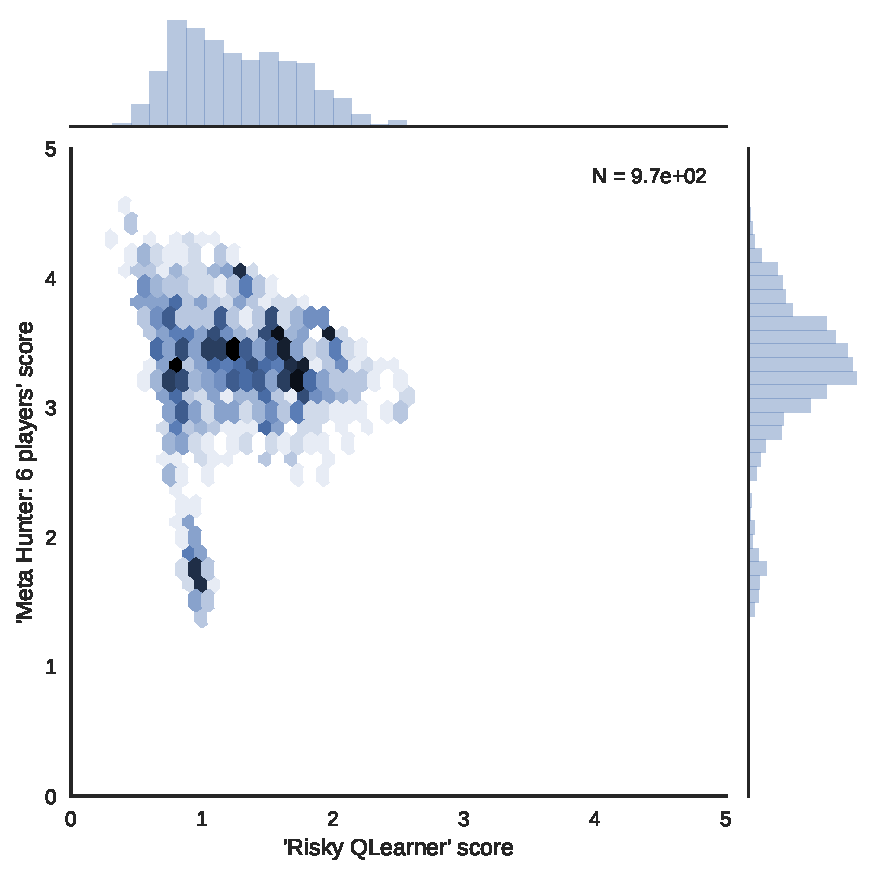
\includegraphics[width=.4\textwidth]{../img/players_with_most_scores.pdf}
    \caption{All possible scores for the pair of strategies that have the most
    different number of match outcomes}
    \label{fig:players_with_most_scores}
\end{figure}

\section{Validation}\label{sec:validation}

As described in \cite{Nowak} Consider the payoff matrix:

\begin{equation}\label{equ:payoff_matrix}
    M = \begin{pmatrix}
        a, b\\
        c, d
        \end{pmatrix}
\end{equation}

The expected payoffs of \(i\) players of the first type in a population with \(N
- i\) players of the second type are given by:

\begin{equation}\label{equ:expected_payoff_one}
    F_i = \frac{a(i - 1) + b(N - i)}{N - 1}
\end{equation}

\begin{equation}\label{equ:expected_payoff_two}
    G_i = \frac{ci + d(N - i - 1)}{N - 1}
\end{equation}

With an intensity of selection \(\omega\) the fitness of both strategies is
given by:

\begin{equation}\label{equ:expected_payoff_one}
    f_i = 1 - \omega + \omega F_i
\end{equation}

\begin{equation}\label{equ:expected_payoff_two}
    g_i = 1 - \omega + \omega G_i
\end{equation}

The transitions within the birth death process that underpins the Moran process
are then given by:

\begin{align}
	p_{i, i+1}&= \frac{if_i}{if_i+(N-i)g_i}\frac{N-i}{N}\label{equ:p_up}\\
	p_{i, i-1}&= \frac{(N-i)g_i}{if_i+(N-i)g_i}\frac{i}{N}\label{equ:p_down}\\
	p_{ii} &= 1 - p_{i, i+1} - p_{i, i-1}\label{equ:p_stay}
\end{align}

Using this it is a known result that the fixation probability of the first
strategy in a population of \(i\) individuals of the first type (and \(N-i\)
individuals of the second. We have:

\begin{equation}\label{equ:fixation_probability}
x_i = \frac{1 + \sum_{j=1}^{i-1}\prod_{k=1}^{j}\gamma_j}{1 + \sum_{j=1}^{N-1}\prod_{k=1}^{j}\gamma_j}
\end{equation}

where:

\[
\gamma_j = \frac{p_{j, j-1}}{p_{j, j+1}}
\]

Using this comparisons of \(x_{N/2}\) are shown in
Figure~\ref{fig:comparison_deterministic}. Note that these are all deterministic
strategies and show a perfect match up between the expected value of
(\ref{equ:fixation_probability}) and the actual Moran process.

\begin{figure}[!hbtp]
    \centering
    \begin{subfigure}[t]{.3\textwidth}
        \centering
        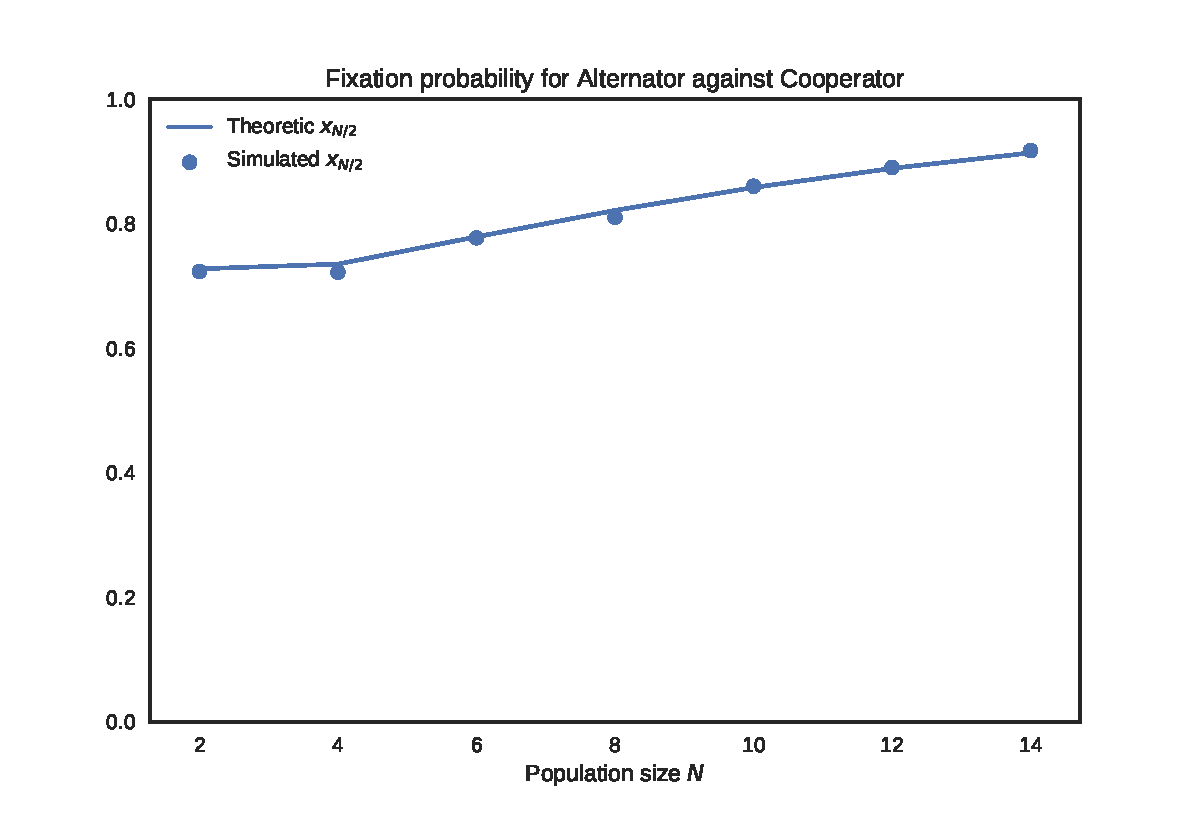
\includegraphics[width=.8\textwidth]{../img/Alternator_v_Cooperator_1000_repetitions.pdf}
        \caption{Alternator and Cooperator}
    \end{subfigure}%
    ~
    \begin{subfigure}[t]{.3\textwidth}
        \centering
        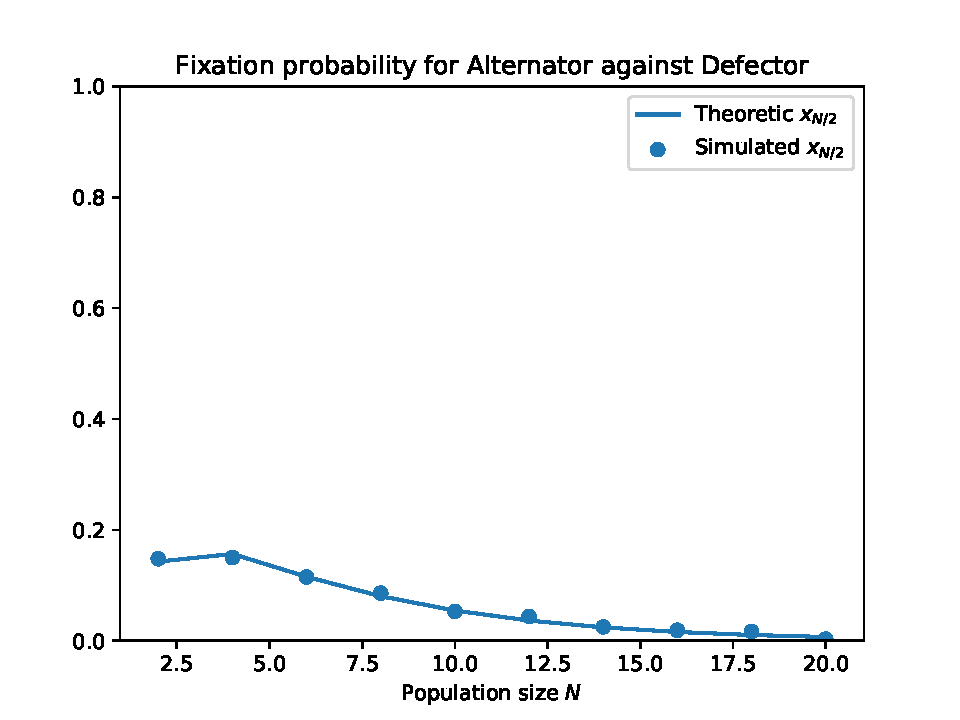
\includegraphics[width=.8\textwidth]{../img/Alternator_v_Defector_1000_repetitions.pdf}
        \caption{Alternator and Defector}
    \end{subfigure}%
    ~
    \begin{subfigure}[t]{.3\textwidth}
        \centering
        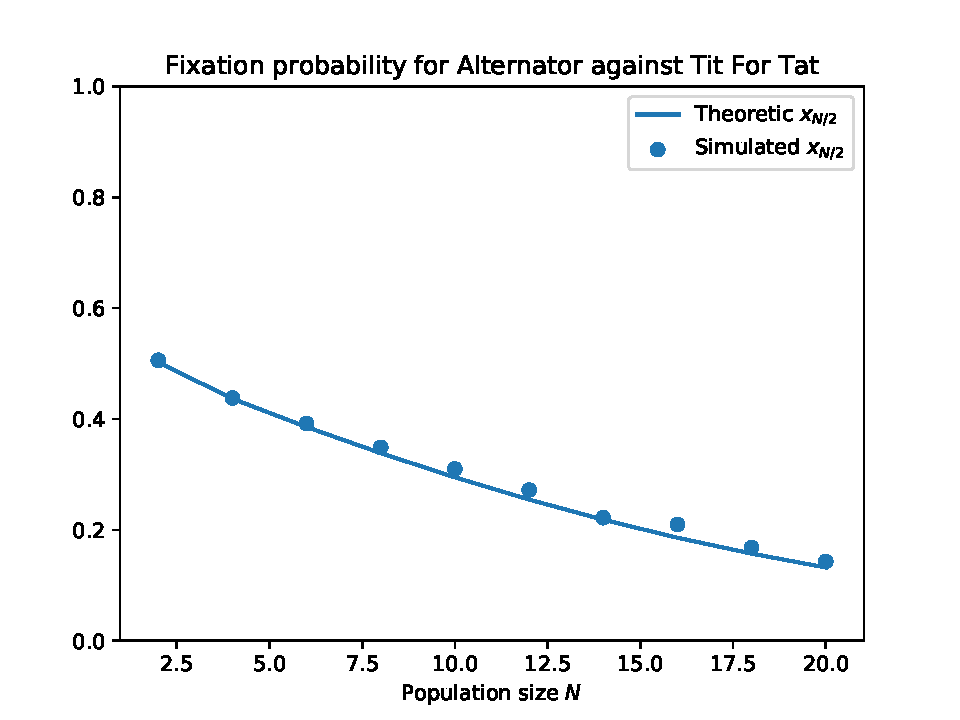
\includegraphics[width=.8\textwidth]{../img/Alternator_v_Tit_For_Tat_1000_repetitions.pdf}
        \caption{Alternator and Tit For Tat}
    \end{subfigure}%

    \begin{subfigure}[t]{.3\textwidth}
        \centering
        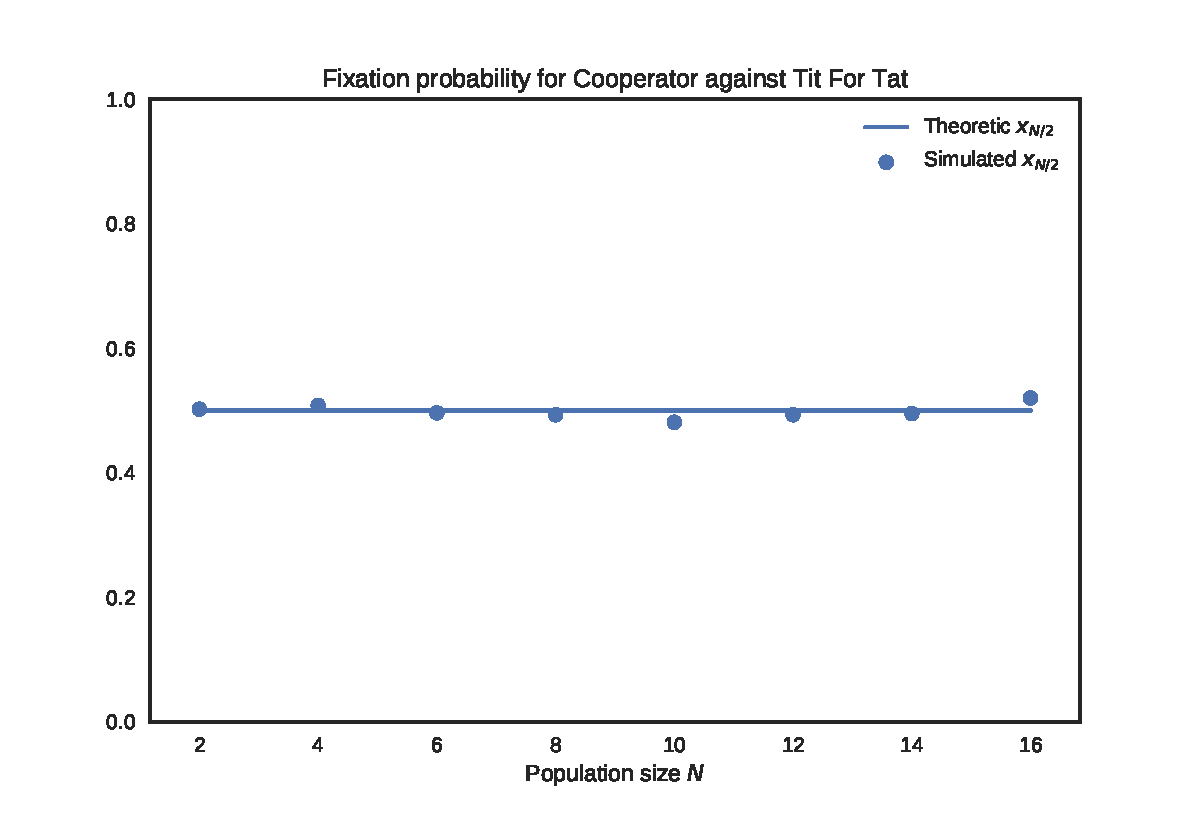
\includegraphics[width=.8\textwidth]{../img/Cooperator_v_Tit_For_Tat_1000_repetitions.pdf}
        \caption{Cooperator and Tit For Tat}
    \end{subfigure}%
    ~
    \begin{subfigure}[t]{.3\textwidth}
        \centering
        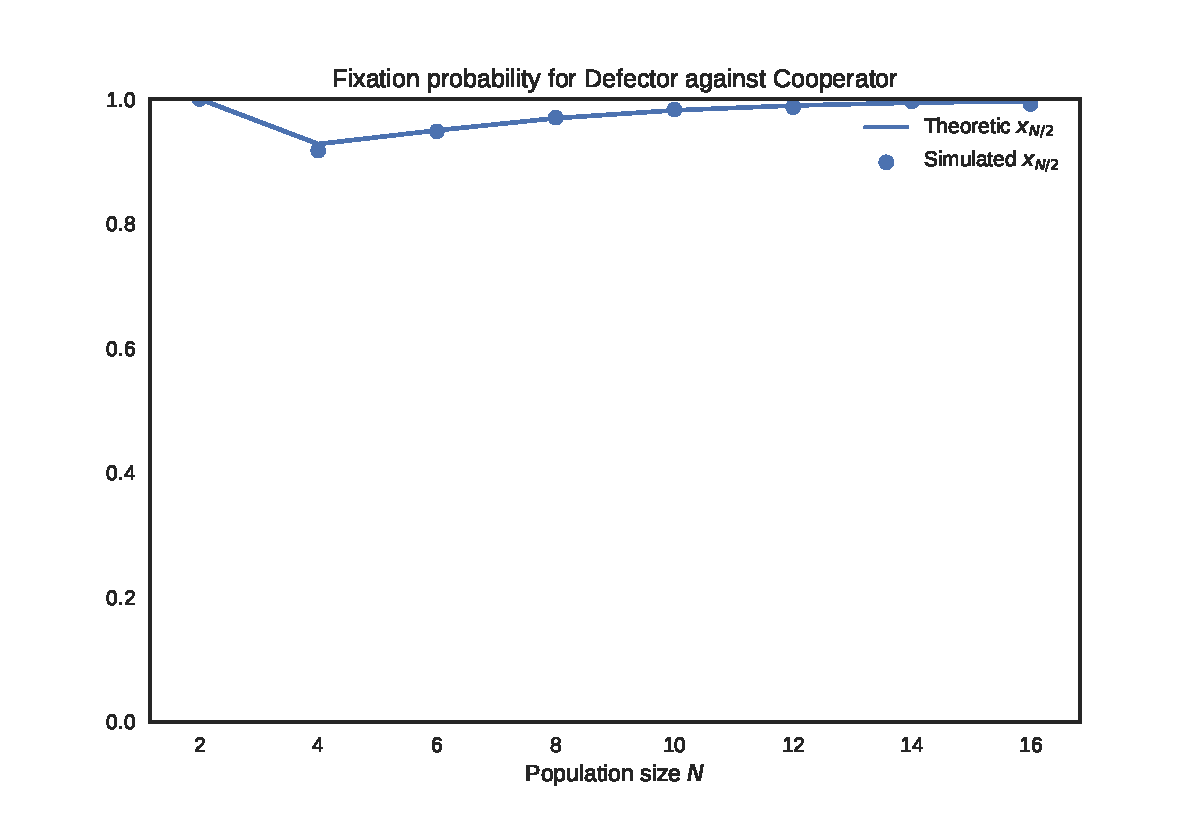
\includegraphics[width=.8\textwidth]{../img/Defector_v_Cooperator_1000_repetitions.pdf}
        \caption{Defector and Cooperator}
    \end{subfigure}%
    ~
    \begin{subfigure}[t]{.3\textwidth}
        \centering
        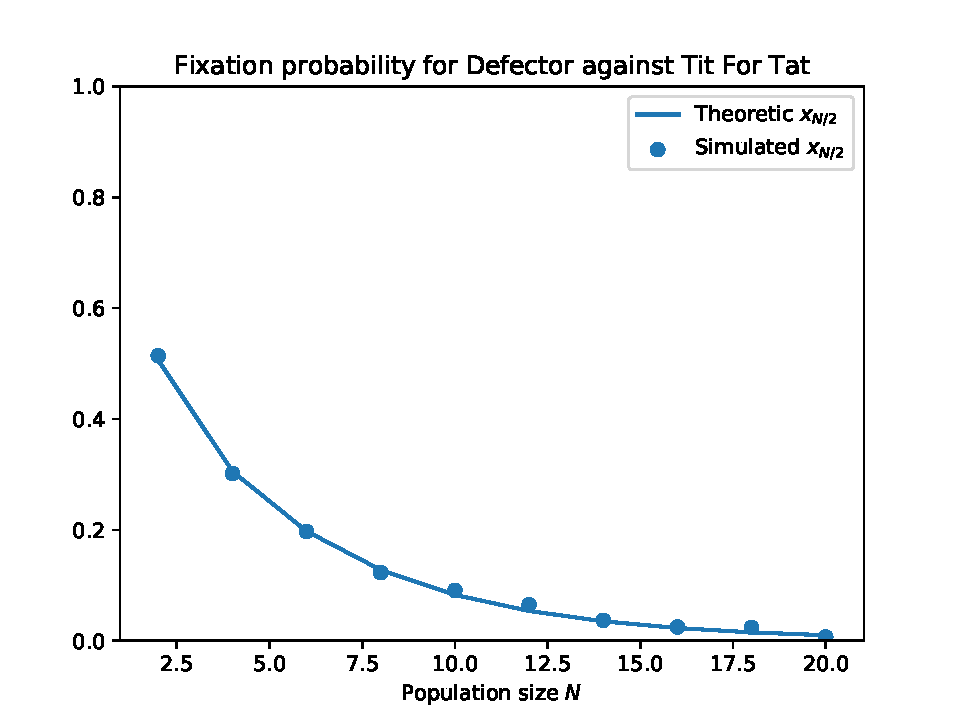
\includegraphics[width=.8\textwidth]{../img/Defector_v_Tit_For_Tat_1000_repetitions.pdf}
        \caption{Defector and Tit For Tat}
    \end{subfigure}%
    \caption{Comparison of theoretic and actual Moran Process fixation probabilities for \textbf{deterministic} strategies}
    \label{fig:comparison_deterministic}
\end{figure}

\begin{figure}[!hbtp]
    \centering
    \begin{subfigure}[t]{.3\textwidth}
        \centering
        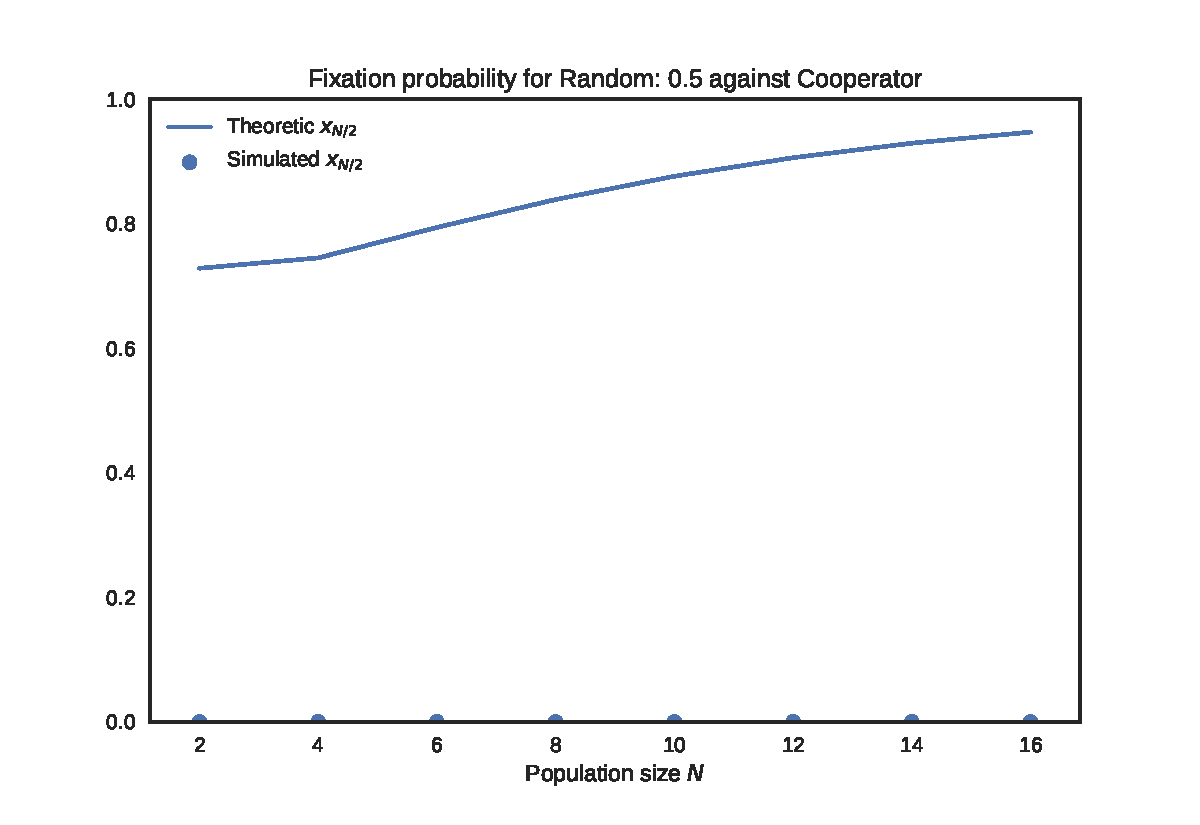
\includegraphics[width=.8\textwidth]{../img/Random_0_5_v_Cooperator_1000_repetitions.pdf}
        \caption{Random and Cooperator}
    \end{subfigure}%
    ~
    \begin{subfigure}[t]{.3\textwidth}
        \centering
        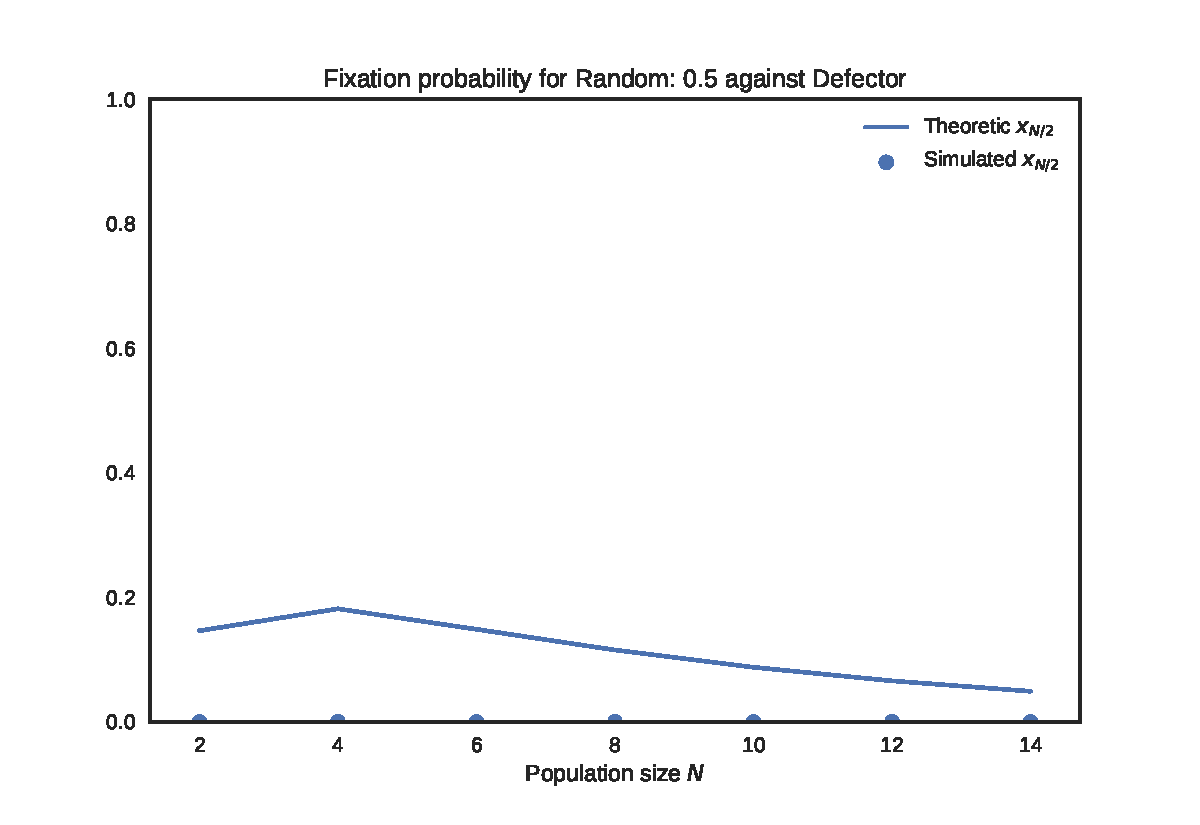
\includegraphics[width=.8\textwidth]{../img/Random_0_5_v_Defector_1000_repetitions.pdf}
        \caption{Random and Defector}
    \end{subfigure}%
    ~
    \begin{subfigure}[t]{.3\textwidth}
        \centering
        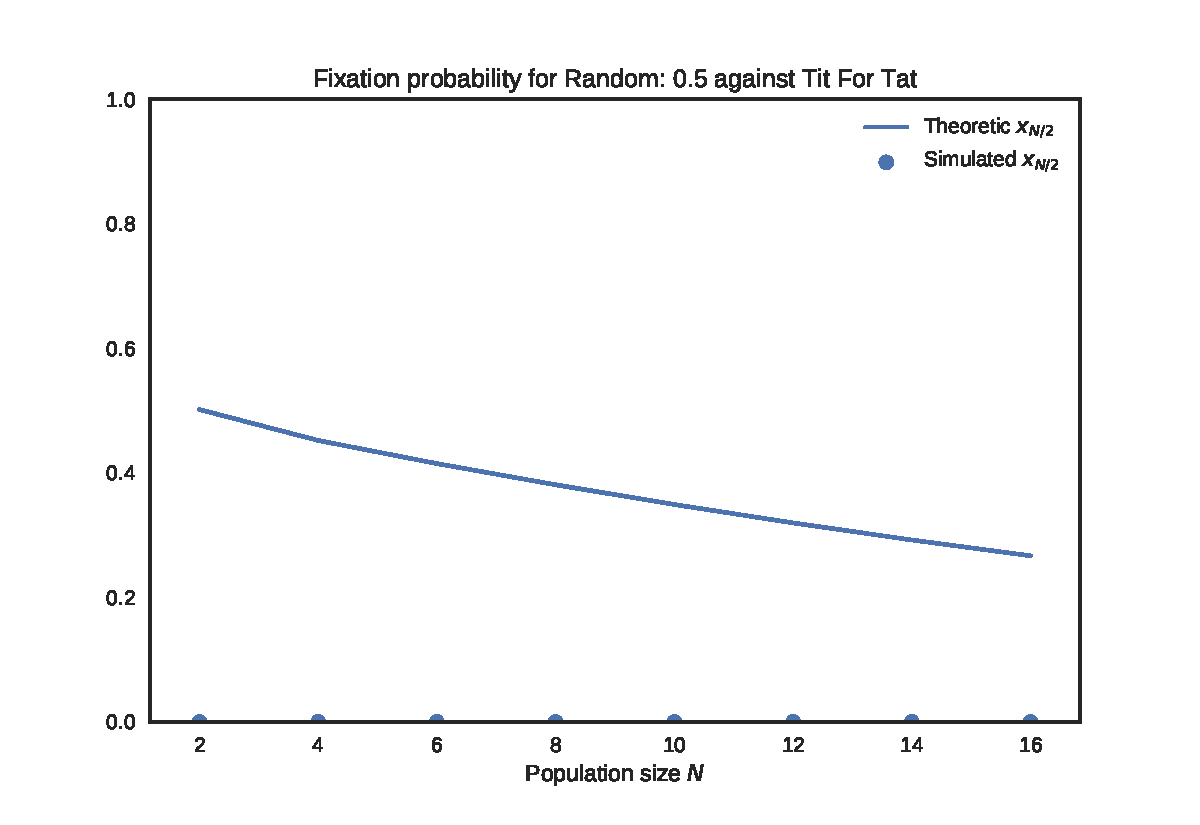
\includegraphics[width=.8\textwidth]{../img/Random_0_5_v_Tit_For_Tat_1000_repetitions.pdf}
        \caption{Random and Tit For Tat}
    \end{subfigure}%
    % TODO Input more of these
    \caption{Comparison of theoretic and actual Moran Process fixation probabilities for \textbf{stochastic} strategies}
    \label{fig:comparison_stochastic}
\end{figure}

Figure~\ref{fig_comparison_stochastic} shows the fixation probabilities for
stochastic strategies. These are no longer a good match which highlights the
weakness of the analytical formulae the relies on the average payoffs. A
detailed analysis of the 172 strategies considered will be shown in the next
Section.

\section{Numerical results}\label{sec:numerical_results}

Structure:

\begin{itemize}
    \item General overview of the data obtained;
    \item Inclusion of most of the work in \texttt{Moran.ipynb}.
\end{itemize}

\section{Conclusion}\label{sec:conclusion}

\printbibliography

\appendix

\section{List of players}\label{app:list_of_players}

\begin{multicols}{3}
	\begin{enumerate}
		\item Hard Tit For Tat
\item Negation
\item Nice Average Copier
\item Nydegger
\item Winner21
\item Winner12
\item $\pi$
\item Win-Shift Lose-Stay: D
\item Omega TFT: 3, 8
\item Opposite Grudger
\item FSM Player: [(0, 'C', 13, 'D'), (0, 'D', 12, 'D'), (1, 'C', 3, 'D'), (1, 'D', 4, 'D'), (2, 'C', 14, 'D'), (2, 'D', 9, 'D'), (3, 'C', 0, 'C'), (3, 'D', 1, 'D'), (4, 'C', 1, 'D'), (4, 'D', 2, 'D'), (5, 'C', 12, 'C'), (5, 'D', 6, 'C'), (6, 'C', 1, 'C'), (6, 'D', 14, 'D'), (7, 'C', 12, 'D'), (7, 'D', 2, 'D'), (8, 'C', 7, 'D'), (8, 'D', 9, 'D'), (9, 'C', 8, 'D'), (9, 'D', 0, 'D'), (10, 'C', 2, 'C'), (10, 'D', 15, 'C'), (11, 'C', 7, 'D'), (11, 'D', 13, 'D'), (12, 'C', 3, 'C'), (12, 'D', 8, 'D'), (13, 'C', 7, 'C'), (13, 'D', 10, 'D'), (14, 'C', 10, 'D'), (14, 'D', 7, 'D'), (15, 'C', 15, 'C'), (15, 'D', 11, 'D')], 1, C
\item Once Bitten
\item Predator
\item FSM Player: [(0, 'C', 0, 'C'), (0, 'D', 3, 'C'), (1, 'C', 5, 'D'), (1, 'D', 0, 'C'), (2, 'C', 3, 'C'), (2, 'D', 2, 'D'), (3, 'C', 4, 'D'), (3, 'D', 6, 'D'), (4, 'C', 3, 'C'), (4, 'D', 1, 'D'), (5, 'C', 6, 'C'), (5, 'D', 3, 'D'), (6, 'C', 6, 'D'), (6, 'D', 6, 'D'), (7, 'C', 7, 'D'), (7, 'D', 5, 'C')], 1, C
\item Prober 2
\item Prober
\item Prober 3
\item Tricky Defector
\item Tullock: 11
\item VeryBad
\item Prober 4
\item Willing
\item Worse and Worse 2
\item Pun1
\item Two Tits For Tat
\item Tricky Cooperator
\item PSO Gambler 2\_2\_2
\item PSO Gambler 1\_1\_1
\item Tit For Tat
\item Worse and Worse
\item ZD-Extort-2: 0.1111111111111111, 0.5
\item Worse and Worse 3
\item Win-Stay Lose-Shift: C
\item Hard Tit For 2 Tats
\item Tit For 2 Tats
\item Hard Go By Majority
\item Cycle Hunter
\item Fool Me Once
\item ZD-GTFT-2: 0.25, 0.5
\item Adaptive
\item Cooperator Hunter
\item Forgiving Tit For Tat
\item Handshake
\item Eventual Cycle Hunter
\item Retaliate 3: 0.05
\item Forgetful Fool Me Once: 0.05
\item Adaptive Tit For Tat: 0.5
\item Forgiver
\item Revised Downing: True
\item Evolved ANN
\item Forgetful Grudger
\item Hard Go By Majority: 10
\item PSO Gambler 2\_2\_2 Noise 05
\item Cycler CCCCCD
\item Ripoff
\item Aggravater
\item Evolved ANN 5
\item Fortress3
\item Hard Go By Majority: 20
\item ZD-GEN-2: 0.125, 0.5, 3
\item ALLCorALLD
\item Hard Prober
\item Evolved ANN 5 Noise 05
\item SelfSteem
\item Alternator
\item Fortress4
\item Hard Go By Majority: 40
\item Cycler CCCD
\item Risky QLearner
\item FSM Player: [(0, 'C', 7, 'C'), (0, 'D', 1, 'C'), (1, 'C', 11, 'D'), (1, 'D', 11, 'D'), (2, 'C', 8, 'D'), (2, 'D', 8, 'C'), (3, 'C', 3, 'C'), (3, 'D', 12, 'D'), (4, 'C', 6, 'C'), (4, 'D', 3, 'C'), (5, 'C', 11, 'C'), (5, 'D', 8, 'D'), (6, 'C', 13, 'D'), (6, 'D', 14, 'C'), (7, 'C', 4, 'D'), (7, 'D', 2, 'D'), (8, 'C', 14, 'D'), (8, 'D', 8, 'D'), (9, 'C', 0, 'C'), (9, 'D', 10, 'D'), (10, 'C', 8, 'C'), (10, 'D', 15, 'C'), (11, 'C', 6, 'D'), (11, 'D', 5, 'D'), (12, 'C', 6, 'D'), (12, 'D', 9, 'D'), (13, 'C', 9, 'D'), (13, 'D', 8, 'D'), (14, 'C', 8, 'D'), (14, 'D', 13, 'D'), (15, 'C', 4, 'C'), (15, 'D', 5, 'C')], 1, C
\item Meta Hunter Aggressive: 7 players
\item Alternator Hunter
\item Evolved FSM 4
\item Cycler CCD
\item Slow Tit For Two Tats 2
\item $e$
\item Soft Go By Majority
\item Hard Go By Majority: 5
\item ShortMem
\item AntiCycler
\item Hesitant QLearner
\item Cycler DC
\item Evolved FSM 16
\item GTFT: 0.33
\item Slow Tit For Two Tats
\item Anti Tit For Tat
\item Shubik
\item General Soft Grudger: n=1,d=4,c=2
\item Soft Grudger
\item ZD-Extort-2 v2: 0.125, 0.5, 1
\item Soft Go By Majority: 10
\item Hopeless
\item Adaptive Pavlov 2006
\item Sneaky Tit For Tat
\item Inverse
\item Cycler DDC
\item Evolved FSM 16 Noise 05
\item Adaptive Pavlov 2011
\item Soft Go By Majority: 20
\item Inverse Punisher
\item PSO Gambler Mem1
\item SolutionB5
\item Appeaser
\item EvolvedLookerUp2\_2\_2
\item Joss: 0.9
\item Cycler CCCDCD
\item EvolvedLookerUp1\_1\_1
\item Punisher
\item Soft Go By Majority: 40
\item SolutionB1
\item Arrogant QLearner
\item Soft Go By Majority: 5
\item Defector
\item Level Punisher
\item Spiteful Tit For Tat
\item Raider
\item Soft Joss: 0.9
\item Meta Hunter: 6 players
\item Average Copier
\item Davis: 10
\item Limited Retaliate: 0.1, 20
\item Stochastic Cooperator
\item ZD-Extort-4: 0.23529411764705882, 0.25, 1
\item $\phi$
\item ZD-SET-2: 0.25, 0.0, 2
\item Better and Better
\item Limited Retaliate 2: 0.08, 15
\item Defector Hunter
\item Random Hunter
\item Stochastic WSLS: 0.05
\item Gradual
\item Limited Retaliate 3: 0.05, 20
\item Random: 0.5
\item Retaliate 2: 0.08
\item Remorseful Prober: 0.1
\item Suspicious Tit For Tat
\item Bully
\item Desperate
\item Gradual Killer: ('D', 'D', 'D', 'D', 'D', 'C', 'C')
\item Tester
\item CollectiveStrategy
\item Math Constant Hunter
\item Firm But Fair
\item Grofman
\item Feld: 1.0, 0.5, 200
\item ThueMorse
\item Cautious QLearner
\item Naive Prober: 0.1
\item Resurrection
\item Doubler
\item Fool Me Forever
\item Grudger
\item ThueMorseInverse
\item Evolved HMM 5
\item GrudgerAlternator
\item MEM2
\item Retaliate: 0.1
\item Contrite Tit For Tat
\item EasyGo
\item Calculator
\item Grumpy: Nice, 10, -10
\item Thumper
\item Cooperator
\item Eatherley

	\end{enumerate}
\end{multicols}

\end{document}
